\documentclass[12pt]{article}
\usepackage[utf8]{inputenc}
\usepackage{algorithmic}
\usepackage{amsmath}
\usepackage{amssymb}
\usepackage{amsfonts}
\usepackage[margin=1in]{geometry}
\usepackage{graphicx} 
\usepackage{hyperref}
\graphicspath{ {images/} }
\setlength{\parskip}{\baselineskip}%
\setlength{\parindent}{0pt}%
\graphicspath{ {images/} }
\title{Probability and Statistics \\ Assignment R}
\author{Hien Le - 11186429 - hien.le@student.auc.nl \\ Deniz Ovalioglu - }
\date{March 2018}

\begin{document}
\maketitle

\subsection*{Exercise R.1}
Suppose a coin is flipped repeatedly for which the probability of
heads is $p = 0.3$. Different flips of the coin are independent. In what follows, $X_{n}$ denotes the number of heads obtained after $n$ flips.

(a) Based on the frequency interpretation of the concept “probability”, what value would you expect $X_{n}$ to have when $n$ is large?
\subsubsection*{Answer}
Based on the description of $X_{n}$, we can deduce that $X_{n}$ has a Binomial distribution i.e. $X_{n} \sim Bin(n, 0.3)$. Therefore, when $n$ is large, the expectation of $X_{n}$ will be 0.3$n$. The reasoning can be seen in the calculation below:\\
Let $X \sim Bin(n,p)$, when $n$ is large, $X \sim E(X) = E\Sigma^{n}_{i=1}X_{i} = \Sigma^{n}_{i=1}E(X_{i}) = np$.

(b) Simulate in R a series of 500 coin flips. Make a plot of $X_{n}$ against $n$, for $n = 1, . . . , 500$. Use \texttt{type="l"} for plotting. Add to this plot the line $np$ against $n$, in a different color.
Hint: A series of 500 independent coin flips can be generated by the R-
command \texttt{x=rbinom(500,1,p)}. The R-function \texttt{cumsum} can be useful when you determine the number of heads after n flips.
\subsubsection*{Answer}
Plot:

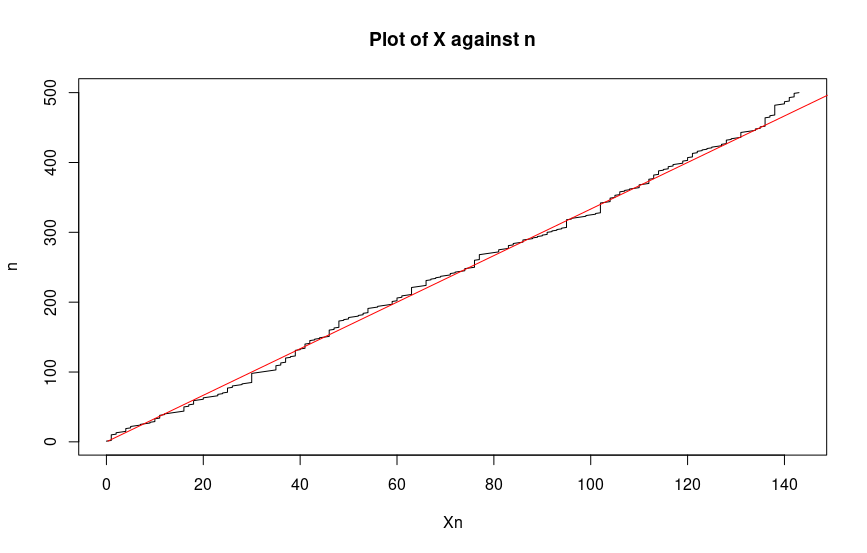
\includegraphics[width=\textwidth]{Ex1Plot1}

(c) Investigate how close the two graphs you produced in part (b) are, relative to their height. That is, for every $n$, compute the relative error
$\frac{|X_{n} - np|}{np}$. What happens to the relative error as the number of flips grows? Is this in accordance with your expectations in part (a)?
\subsubsection*{Answer}
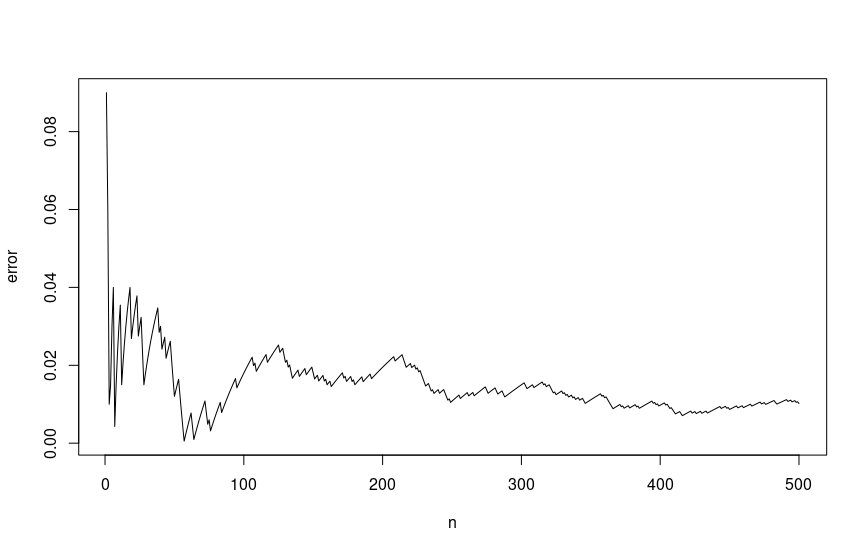
\includegraphics[width=\textwidth]{Ex1Plot2}

Looking at the plot above, it can be concluded that the error reduces as the number of flips grows. This is in accordance with part a, which claims that as $n$ becomes large, the value of $X_{n}$ eventually reaches $np$.

\subsection*{Exercise R.2}
(a) Make exercise 2.18 (a)–(d) of the book using R (do not use the Normal table). Now simulate in R six random samples from $N(3, 16)$: two of size 20, two of size 100, two of size 1.000.

(b) Determine for each of the six samples:\\
- the proportion of values that are smaller than 7;\\
- the proportion of values larger than -2;\\
- the 0.95-sample quantile, i.e. the smallest value in the sample for which it holds that at most 1\% of the data in the sample is larger than or equal to this value (use the R-function quantile with \texttt{type=1}).
- the proportion of values larger than or equal to 0 and smaller than 4.

Present your results of parts (a) and (b) together in one table. Round all the values to three decimal places.

(c) Compare your results for the six samples of part (b) to each other and to the corresponding answers of part (a). Briefly comment on your findings.

(d) For each of the six samples, draw the scaled histogram and draw the probability density function of $N(3, 16)$ on top of it. Present the six plots in one figure. Briefly comment on what you see in the plots.\\
Hint: The p.d.f. of a normal distribution in R is the function \texttt{dnorm}.

(e) Which common phenomenon do your findings in parts (c) and (d) illustrate?

\subsection*{Exercise R.3}
In this exercise, you will estimate an unknown probability by the frequency of occurrence of the event in a long series of experiments. Assume that birthdays are uniformly spread over a year of 365 days, and that $n$ students are chosen at random independently from each other. Consider the event $A_{n}$ = {there is a day (at least one) in the year when at least 3 out of the $n$ chosen students have their birthday}.

(a) Write a function that estimates $P\{A_{n}\}$ by simulating 100 experiments (that is, by taking 100 samples of size $n$) and finding out for each experiment (that is, for each sample) if $A_n$ occurs. Take $n$ as the argument of the function.\\
Hint: Use a for-loop.
\subsubsection*{Answer}
See Appendix for Exercise R.3

(b) Create a vector prob that consists of the estimates for the probabilities $P\{A_{n}\}$ for $n = 1, 2, . . . , 200$. Plot these probabilities against $n$.
\subsubsection*{Answer}
Plot:

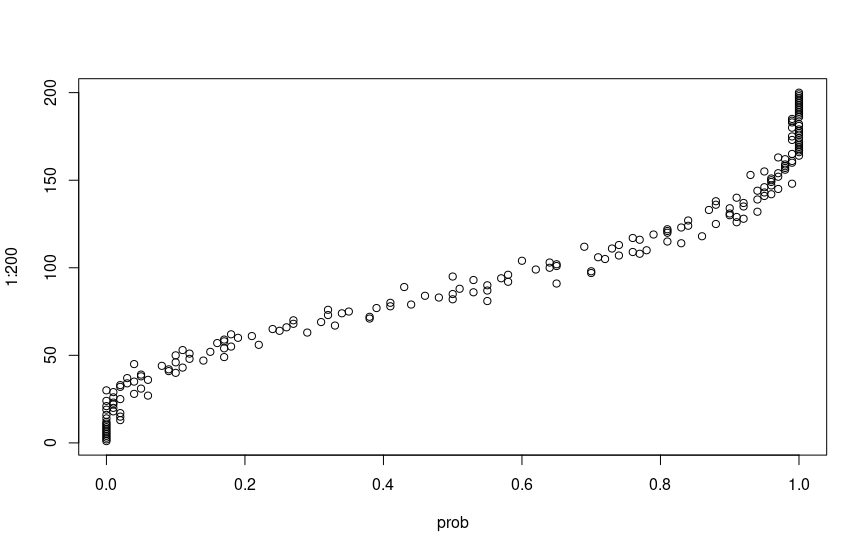
\includegraphics[width=\textwidth]{Ex3Plot1}

(c) Estimate the number of students that should be chosen so that the probability of the event $A_{n}$ is at least 70\% by finding the smallest $n$ such that prob[$n$] $\geq$ 0.7.\\
\subsubsection*{Answer}
See the code in Appendix for Exercise R.3.

The smallest $n$ that was returned from 100 experiments of 200 students in each was 102.

(d) Do you think it is really the case that $P\{A_{n}\} \geq$ 0.7 for the $n$ you found in part (c)? Check your answer by making a new estimate for $P\{A_{n}\}$ based on 10.000 samples and comment.
\subsubsection*{Answer}
For 10,000 samples, the least $n$ found was [to insert result here]

(e) Take 100 samples of 75 students, and for each sample count on how many days at least 3 students celebrate their birthday simultaneously. Make a histogram of these numbers and calculate the average.
\subsubsection*{Answer}
Plot:

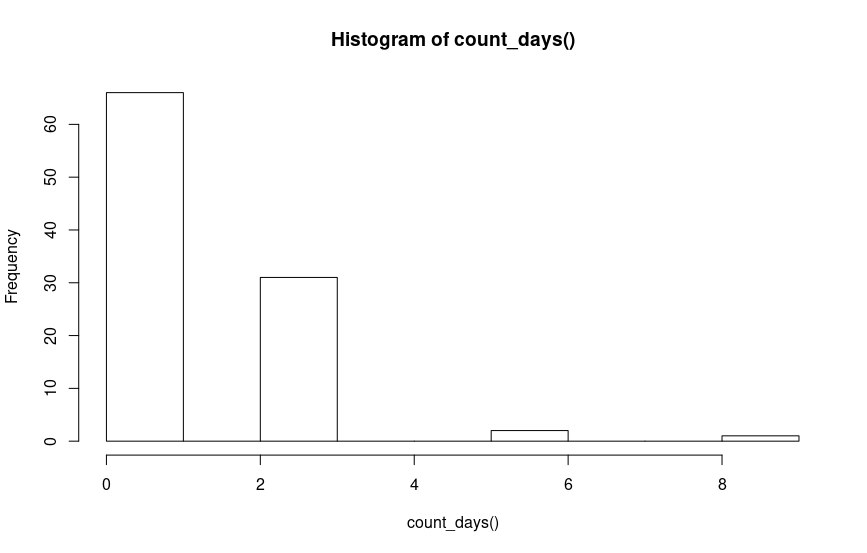
\includegraphics[width=\textwidth]{Ex3Plot2}

(f) Repeat the calculation of part (e) 100 times and make a histogram of the averages. Compare to the histogram from part (e) and comment.
\subsubsection*{Answer}
Plot:

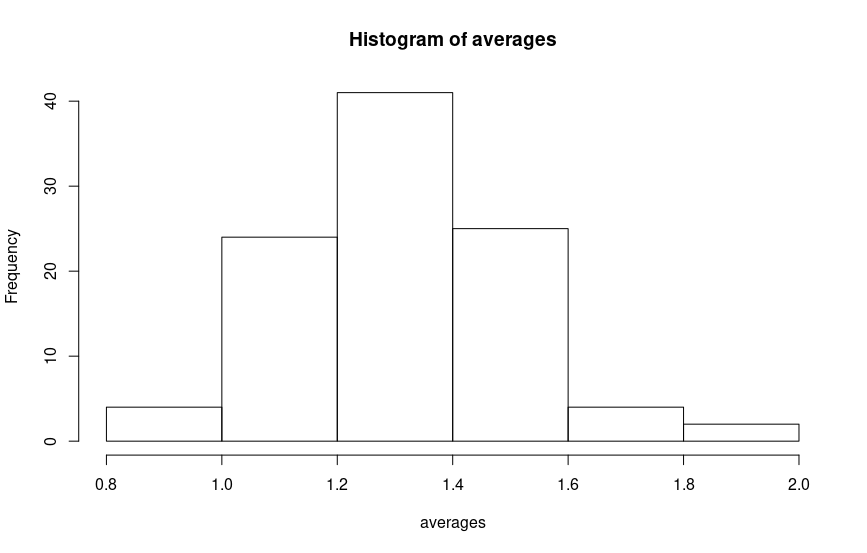
\includegraphics[width=\textwidth]{Ex3Plot3}
As can be seen, the two diagrams differ greatly. [to elaborate here]

\subsection*{Exercise R.4}
R has commands that generate random variables from many standard distributions. In this exercise, you will learn how to simulate random variables from non-standard distributions. Consider the following c.d.f.:

$F(x) = \frac{e^{x}}{1 + e^{x}}$, $x \in R$

(a) Compute the quantile function $F^{-1}(q), q \in (0, 1)$.

(b) Simulate a random sample u of size $n = 1.000$ from the uniform distribution on (0, 1). Apply the quantile function $F^{-1}$ to u element-wise and plot a scaled histogram of this transformed vector.\\
Hint: A sample of size n from the uniform distribution on $(a, b)$ can be generated by the R-command \texttt{runif(n,a,b)}.

(c) Compute the p.d.f. that corresponds to $F$ and plot it on top of the histogram from (b).

(d) Let a random variable U have uniform distribution on (0, 1). Prove that the c.d.f. of $F^{-1}(U) is F$.\\
Hint: The events ${F^{-1}(U) \leq x}$ and ${F(F^{-1}(U)) \leq F(x)}$ are the same, why?

(e) Based on the previous parts of the exercise, how can you simulate a random variable with the c.d.f. $F$ in R? Which of the previous parts of the exercise proves this approach works and which part illustrates this approach works?

(f) Which properties of $F$ enable the approach from (e) to work? Would this approach work for other c.d.f.’s with these properties?

\subsection*{Appendix}

\subsubsection*{Exercise R.1}
\begin{verbatim}

# R.1.b
coin_flips = rbinom(500, 1, 0.3)
range_n = 500
generate_plot= function(sample, n, p){
  plot(cumsum(sample), n, xlab="Xn", ylab="n", main="Plot of X against n", type="l")
  lines(n*p, n, col="red", type="l")
}

#generate_plot(coin_flips, 1:range_n, 0.3)

# R.1.c
get_relative_error = function(sample, n, p){
  vector_n = c(1:n)
  error_vector = abs(cumsum(sample) - vector_n*p)/vector_n*p
  plot(vector_n, error_vector, xlab="n", ylab="error", type="l")
}

#get_relative_error(coin_flips, 500, 0.3)
\end{verbatim}

\subsubsection*{Exercise R.3}
\label{sec:r.3}
\begin{verbatim}

# R.3.a
birthday_experiments = function(n, expes){
  occurences = 0
  for(i in 1:expes){
    sam = sample(1:365, n, replace=TRUE)
    event_An = FALSE
    for(j in 1:365){ # a bit inefficent => to change
      if(sum(sam==j) >= 3){
        event_An = TRUE
      }
    }
    if(event_An){
      occurences = occurences + 1
    }
  }
  return(occurences/expes)
}

#print(birthday_experiments(200, 100))

# R.3.b
prob = numeric(200)
for(i in 1:200){
  prob[i] = birthday_experiments(i, 100)
}
#print(prob)

plot(prob, 1:200)

# R.3.c
estimate_n = function(n, expes){
  prob = numeric(n)
  least_n = 1
  for(i in 1:n){
    prob[i] = birthday_experiments(i, expes)
  }
  while(prob[least_n] < 0.7){
    least_n = least_n + 1
  }
  print(least_n)
}

estimate_n(200, 100)

# R.3.e
count_days = function(){
  vec_days = numeric(100)
  for(i in 1:100){
    sam = sample(1:365, 75, replace=TRUE)
    num_days = 0
    for(day in sam){
      occurences = length(which(sam==day))
      if(occurences > 2){
        num_days = num_days + 1
      }
    }
    vec_days[i] = num_days
  }
  return(vec_days)
}

#hist(count_days())

# R.3.f
averages = numeric(100)
for(i in 1:100){
  averages[i] = mean(count_days())
}
#hist(averages)

\end{verbatim}
\end{document}